\documentclass[oneside,11pt,letter]{article}

% General include (DO NOT MODIFY)
\usepackage{amsmath,graphicx,cite,latexsym,color, amssymb,ifthen,verbatim}

\usepackage{listings, url}
\definecolor{mygreen}{rgb}{0,0.6,0}
\definecolor{mygray}{rgb}{0.5,0.5,0.5}
\definecolor{mymauve}{rgb}{0.58,0,0.82}

\lstset{ %
  backgroundcolor=\color{white},   % choose the background color
  basicstyle=\footnotesize,        % size of fonts used for the code
  breaklines=true,                 % automatic line breaking only at whitespace
  captionpos=b,                    % sets the caption-position to bottom
  commentstyle=\color{mygreen},    % comment style
  escapeinside={\%*}{*)},          % if you want to add LaTeX within your code
  keywordstyle=\color{blue},       % keyword style
  stringstyle=\color{mymauve},     % string literal style
}
\lstset{basicstyle=\small\ttfamily,breaklines=true}

%--------------- Various Style Declarations ----------------------------
\textheight 9in
\topmargin 0in
\headheight 0in
\headsep 0in
\textwidth 6.5in
\oddsidemargin 0in
\evensidemargin 0in
\footskip 0.2in
\parskip 5pt
\parindent 0pt
\topsep 2pt
\partopsep 0pt
\itemsep 0pt
\pagenumbering{arabic}

\definecolor{shade}{gray}{0.85}


\newcommand{\solpagesize}%
{\ifthenelse{\equal{\type}{solutions}}{
\textheight9in
\textwidth6.5in
\oddsidemargin0in
\evensidemargin0in
\topmargin-0.75in
\topskip0in
\footskip0.70in
\pagestyle{empty}
\parskip 5pt
\parindent 0pt
}{}}

\newcommand{\bookletskip}[1] %
{\ifthenelse{\equal{\type}{booklet}}{\vspace{#1 in}}
}

\newcommand{\bookletpage} %
{\ifthenelse{\equal{\type}{booklet}}{\newpage}{}
}

\newcommand{\inbooklet}[1]{\ifthenelse{\equal{\type}{booklet}}{{#1}}}


%%%%%%%%%%%%%%%%%%%%%%%%%%%%%%%%%%%%%%%
% Here are the new definitions of the commands \problem (for main
% text of problem), \problempart (for parts (a), (b) etc of the problem
% and \solution (for text of the solution).  The usage is as follows.
%
%    \begin{enumerate}
%    \problem{label}{main text of first problem}
%    \begin{enumerate}
%    \problempart{text of part(a) of first problem}
%
%    \solution{text of solution to part(a)}
%    \problempart{\text of part(b)}
%
%    \solution{text of solution to part (b)}
%
% ..... and so on for succeeding parts
%
%    \end{enumerate}
%
%    \problem{label}{main text of second problem}
%    \begin{enumerate}
%    \problempart{text of part(a)}
%
%    \solution{text of solution to part(a)}
%    \problempart{\text of part(b)}
%
%    \solution{text of solution to part (b)}
%    \end{enumerate}
%    ........ and so on for other problems
%    \end{enumerate}
%
% Please note that there needs to be a blank line separating
% a problempart command and the succeeding solution command;
% else the problem part and the solution are typeset as one
% paragraph when we are printing both the problem and its
% solution.  However, it is OK if a problempart follows a
% previous solution without an intervening blank line.  Some day I will
% waste some time figuring out a way around this problem

\newcommand{\problem}[2]%
{\item\label{#1}%
\ifthenelse{\(\equal{\type}{problems}\)\or\(\equal{\type}{both}\)}%
 {{\bf[#1]\\}#2}{{\bf[#1]}}}
 % The problem name always prints on the first line (in boldface
 % and inside square brackets.  The problem text prints on
 % succeeding lines if we are printing problems only, or problems
 % and solutions both

  \newcommand{\problempart}[1]%
{\item{\ifthenelse{\(\equal{\type}{problems}\)\or\(\equal{\type}{both}\)}%
 {#1}{}}}
 % The tag ((a), or (b) or (c) etc.) of the text of the part of the problem
 % prints in the margin, and is followed by the text of the problem beginning
 % on the same line if we are printing problems only or problems and
 % solutions both

 \newcommand{\solution}[1]%
{\ifthenelse{\equal{\type}{both}}{{\bf{Solution:\ }}{#1}}%
 {\ifthenelse{\(\equal{\type}{solutions}\)}%
 {#1}{}}}
 % This command does not generate a tag ((a), or (b) or (c) etc.)
 % for the text, but uses the tag generated by the previous 
 % problempart or examproblempart command.  If only the solutions 
 % are being printed, then the text
 % of the solution is printed beginning on the same line as the tag.
 % If both problems and solutions are being printed, then "Solution:"
 % is printed in boldface followed by the text of the solution.

  %%%%%%%%%%%%%%%%%%%%%%%%%%%%%%%%%%%%%%%%%
  
  
 \newcommand{\examproblem}[2]%
{\item {\ifthenelse{\equal{\type}{solutions}}{}{{\bf [#1 points]} #2}}}
% The first argument is an integer specifying the number of points.  The
% first argument (followed by the word "points") is printed inside square
% brackets in boldface.  The second argument is the text of the problem
% itself.


\newcommand{\examproblempart}[1]%
{\item{\ifthenelse{\(\equal{\type}{problems}\)\or\(\equal{\type}{both}\)\or\(\equal{\type}{booklet}\)}%
 {#1}{}}}
 % The tag ((a), or (b) or (c) etc.) of the text of the part of the problem
 % prints in the margin, and is followed by the text of the problem beginning
 % on the same line if we are printing problems only or problems and
 % solutions both

%%%%%%%  ENTER SOME PROBLEM SET SPECIFIC STUFF HERE  %%%%



%%%%%%%%%%%%%%%%%%%%%%
%CHANGE
%.   to booklet to print the problems only
%
%    to both to print problems and solutions
%%%%%%%%%%%%%%%%%%%%%%

\newcommand{\type}{booklet}
%\newcommand{\type}{both}

% Custom adjustments (CHANGE THIS FILE FOR ADDITIONAL ADJUSTMENTS)
\usepackage{tikz}
\newcommand{\cN}{{\cal N}}

\DeclareMathOperator*{\argmin}{\arg\!\min}
\newcommand{\norm}[1]{\left\lVert#1\right\rVert}

%************************************************************************
%                                                                       *
%            End of preamble and beginning of text.                     *
%                                                                       *
%************************************************************************

\begin{document}
%------------------------- Title Page ----------------------------------
\thispagestyle{empty}
\baselineskip2.5ex
{\bf University of Illinois}
\hfill
Spring 2018

{\Large
\begin{center}
{\sf CS\,446: Machine Learning}\\ Homework 12\\
\end{center}
}
{\large
\begin{center}
{\color{red}Due on April 24, 2018, 11:59 a.m. Central Time}
\end{center}
}

\ifthenelse{\equal{\type}{booklet}}{}{}

\begin{enumerate}

%%%%%%%%%%%%%%%%%%%%%%%%%%%%%%%%%%%%%%
%%%%%  BEGINNING OF PROBLEMS LIST

%\input{regression}
%\bookletpage
%\input{LinLogReg}
%\bookletpage
%% !TEX root = HW3.tex
\ifthenelse{\equal{\type}{booklet}}{
% !TEX root = HW3.tex

\newcommand{\binStudSolA}{
%%%%%%%%%%%%%%%%%%%%%%%%%%%%%%%%%%%%
%%
%%.   YOUR SOLUTION FOR PROBLEM A BELOW THIS COMMENT
%%
%%%%%%%%%%%%%%%%%%%%%%%%%%%%%%%%%%%%
We simply take the sign of the predicted real value:
\[ y = \text{sign}(\bf{w}^\intercal \bf{x}) \]
}

\newcommand{\binStudSolB}{
%%%%%%%%%%%%%%%%%%%%%%%%%%%%%%%%%%%%
%%
%%.   YOUR SOLUTION FOR PROBLEM B BELOW THIS COMMENT
%%
%%%%%%%%%%%%%%%%%%%%%%%%%%%%%%%%%%%%
Since the sigmoid function maps real numbers to numbers $\in [0, 1]$ its value can be interpreted as a probability. Therefore,
\[
	y = 
	\begin{cases}
		  1 &\quad \text{if g}(\bf{w}^\intercal \bf{x}) > \alpha\\
		-1 &\quad \text{if g}(\bf{w}^\intercal \bf{x}) \le \alpha
	\end{cases}
\]
Where $\alpha \in [0, 1]$ is the threshold chosen. A typical choice is $\alpha = 0.5$.\\

Another way to write this is
\[ y = \text{sign}(\text{g}(\bf{w}^\intercal \bf{x}) - \alpha) \]
}

\newcommand{\binStudSolC}{
%%%%%%%%%%%%%%%%%%%%%%%%%%%%%%%%%%%%
%%
%%.   YOUR SOLUTION FOR PROBLEM C BELOW THIS COMMENT
%%
%%%%%%%%%%%%%%%%%%%%%%%%%%%%%%%%%%%%
Yes. By the chain rule we have that
\begin{align*}
\frac{\partial{g}}{\partial{a}} &= \frac{e^{-a}}{(1 + e^{-a})^2}\\
&= \frac{1}{1 + e^{-a}} \cdot \frac{e^{-a}}{1 + e^{-a}}\\
&= \frac{1}{1 + e^{-a}} \cdot \frac{1 + e^{-a} - 1}{1 + e^{-a}}\\
&= \frac{1}{1 + e^{-a}} \cdot
	 \left( 1 - \frac{1}{1 + e^{-a}} \right) \\
&= g(a) \cdot \left(1 - g(a)\right)
\end{align*}
}

\newcommand{\binStudSolD}{
%%%%%%%%%%%%%%%%%%%%%%%%%%%%%%%%%%%%
%%
%%.   YOUR SOLUTION FOR PROBLEM D BELOW THIS COMMENT
%%
%%%%%%%%%%%%%%%%%%%%%%%%%%%%%%%%%%%%
\newcommand{\wtx}{\mathbf{w}^\intercal \mathbf{x}}
\newcommand{\gxi}{\operatorname{g}\left(\mathbf{w}^\intercal \mathbf{x}_i \right)}
Just like with the least square loss function the update is
\[ \bf{w} = \bf{w} - \alpha \nabla f \]
Where $\nabla f$ is defined as
\[ \nabla f \triangleq \left\langle \frac{\partial{f}}{\partial{\mathbf{w}_k}} \right\rangle_{k=1}^K \]
where $K$ is the number of dimensions. Now,
\[
\frac{
	\partial{f}
}{
	\partial{\mathbf{w}_k}
} = \sum_{i=1} \frac{\partial{f}}{\partial{\gxi}} \cdot \frac{\partial{\gxi}}{\partial{\bf{w}_k}}
\]
But
\[
	\frac{\partial{f}}{\partial{\gxi}} = \gxi - y_i
\]
And
\begin{align*}
\frac{\partial{\gxi}}{\partial{\mathbf{w}_k}} &= 
	\frac{\partial{\gxi}}{\partial{\wtx_i}} \cdot \frac{\partial{\wtx_i}}{\partial{\mathbf{w}_k}}\\
&= \left(
	\operatorname{g}\left( \wtx_i \right)
	\operatorname{g}\left( -\wtx_i \right)
\right) \cdot \mathbf{x}_i^k
\end{align*}

Therefore,
\[
\frac{
	\partial{f}
}{
	\partial{\mathbf{w}_k}
} = \sum_{i=1} \left(
	\left( \gxi - y_i \right)
	\operatorname{g}\left( \wtx_i \right)
	\left(1 - \operatorname{g}\left(\wtx_i \right) \right)
	\mathbf{x}_i^k
\right)
\]
}

\newcommand{\binStudSolE}{
%%%%%%%%%%%%%%%%%%%%%%%%%%%%%%%%%%%%
%%
%%.   YOUR SOLUTION FOR PROBLEM E BELOW THIS COMMENT
%%
%%%%%%%%%%%%%%%%%%%%%%%%%%%%%%%%%%%%
Lets remember that the expression above comes from using the negative log likelihood of the entire dataset. The expression is derived from
\[ \prod_{i} p(y^{(i)} | x^{(i)}) \]
where $p$ follows a logistic distribution.
The above is true \textbf{if} the data samples are i.i.d. That's the assumption made.
}

 %The students have to fill this file to print the solution
}{
}

% Problem Explanation:
% - first argument is the number of points
% - second argument is the title and the text
\examproblem{15}{Binary Classifiers}

%%%%%%%%%%%%%%%%%%%%%%%%%%%%%%%%%%%%%%
%%%%%  BEGINNING OF SUBPROBLEMS LIST
\begin{enumerate}

% Subproblem description
\examproblempart{In order to use a linear regression model for binary classification, how do we map the regression output $\mathbf{w}^\top \mathbf{x}$ to the class labels $y\in\{-1,1\}$? }

% Solution box
\framebox[14.7cm][l]{
\begin{minipage}[b]{14.7cm}

\inbooklet{Your answer: \binStudSolA}

\end{minipage}
}



% Subproblem description
\examproblempart{ In logistic regression, the activation function $\operatorname{g}(a)=\frac{1}{1+e^{-a}}$ is called sigmoid. Then how do we map the sigmoid output $\operatorname{g}(\mathbf{w}^\top \mathbf{x})$ to binary class labels $y\in\{-1,1\}$?}

% Solution box
\framebox[14.7cm][l]{
\begin{minipage}[b]{14.7cm}

\inbooklet{Your answer: \binStudSolB}

\end{minipage}
}



% Subproblem description
\examproblempart{
Is it possible to write the derivative of the sigmoid function $\operatorname{g}$ w.r.t $a$, i.e. $\frac{\partial g}{\partial a}$, as a simple function of itself $\operatorname{g}$? If so, how?
}

% Solution box
\framebox[14.7cm][l]{
\begin{minipage}[b]{14.5cm}

\inbooklet{Your answer: \binStudSolC}

\end{minipage}
}


% Subproblem description
\examproblempart{
Assume quadratic loss is used in the logistic regression together with the sigmoid function. Then the program becomes:
        $$ \min_\mathbf{w} f(\mathbf{w}) := \frac{1}{2} \sum_i \left(y_i - \operatorname{g}(\mathbf{w}^\top \mathbf{x}_i) \right)^2 $$
where $y\in\{0,1\}$. To solve it by gradient descent, what would be the $\mathbf{w}$ update equation?
}

% Solution box
\framebox[14.7cm][l]{
\begin{minipage}[b]{14.5cm}

\inbooklet{Your answer: \binStudSolD}

\end{minipage}
}


% Subproblem description
\examproblempart{
Assume $y\in\{-1,1\}$. Consider the following program for logistic regression:
        $$ \min_\mathbf{w} f(\mathbf{w}) := \sum_i \log\left(1 + \exp(-y^{(i)}\mathbf{w}^T\phi(x^{(i)}))\right).$$
The above program for binary classification makes an assumption on the samples/data points. What is the assumption?}

% Solution box
\framebox[14.7cm][l]{
\begin{minipage}[b]{14.7cm}

\inbooklet{Your answer: \binStudSolE}

\end{minipage}
}


%%%%%%%%%%%% END OF SUBPROBLEMS LIST

\end{enumerate}

%\bookletpage
%\input{svm}
%\bookletpage
%\input{svm2}
%\bookletpage
%% !TEX root = HW6.tex
% !TEX root = HW6.tex

\newcommand{\backpropStudSolA}{
%%%%%%%%%%%%%%%%%%%%%%%%%%%%%%%%%%%%
%%
%%.   YOUR SOLUTION FOR PROBLEM A BELOW THIS COMMENT
%%
%%%%%%%%%%%%%%%%%%%%%%%%%%%%%%%%%%%%
\begin{align*}
g\prime(x) &= \frac{d}{dx}\sigma (x)\\
&= \frac{d}{dx} (1 + e^{-x})^{-1}\\
&= -1 (1 + e^{-x})^{-2}e^{-x}(-1)\\
&= \frac{e^{-x}}{(1 + e^{-x})^{-2}}\\
&= \frac{1}{1 + e^{-x}} \frac{e^{-x}}{1 + e^{-x}}\\
&= \frac{1}{1 + e^{-x}} \frac{1+ e^{-x} - 1}{1 + e^{-x}}\\
&= \frac{1}{1 + e^{-x}} \left( 1 - \frac{1}{1 + e^{-x}} \right)\\
& = \sigma(x) \left(1 - \sigma(x) \right)\\
&= \sigma(x) - \sigma(x)^2
\end{align*}
}

\newcommand{\backpropStudSolB}{
%%%%%%%%%%%%%%%%%%%%%%%%%%%%%%%%%%%%
%%
%%.   YOUR SOLUTION FOR PROBLEM A BELOW THIS COMMENT
%%
%%%%%%%%%%%%%%%%%%%%%%%%%%%%%%%%%%%%
\begin{align*}
\delta_k &= \frac{\partial E}{\partial h_k}\\
&= \frac{\partial}{\partial h_k}
	\frac{1}{2}
	\sum_k \left( c_k - t_k \right)^2\\
&= \frac{\partial}{\partial h_k}
	\frac{1}{2} \left( c_k - t_k \right)^2\\
&= \left( c_k - t_k \right) \frac{\partial}{\partial h_k} c_k\\
&= \left( c_k - t_k \right) \frac{\partial}{\partial h_k} g \left( h_k \right)\\
&=  \left( c_k - t_k \right) g\prime(h_k)
\end{align*}
}

\newcommand{\backpropStudSolC}{
%%%%%%%%%%%%%%%%%%%%%%%%%%%%%%%%%%%%
%%
%%.   YOUR SOLUTION FOR PROBLEM A BELOW THIS COMMENT
%%
%%%%%%%%%%%%%%%%%%%%%%%%%%%%%%%%%%%%
\begin{align*}
\frac{\partial E}{\partial w_{jk}} &= \frac{\partial E}{\partial h_k} \frac{\partial h_k}{\partial w_{jk}}\\
&= \delta_k \frac{\partial h_k}{\partial w_{jk}}\\
&= \delta_k \frac{\partial}{\partial w_{jk}} \sum_j b_j w_{jk} + f_k\\
&= \delta_k \frac{\partial}{\partial w_{jk}} b_j w_{jk}\\
&= \delta_k b_j
\end{align*}
}

\newcommand{\backpropStudSolD}{
%%%%%%%%%%%%%%%%%%%%%%%%%%%%%%%%%%%%
%%
%%.   YOUR SOLUTION FOR PROBLEM A BELOW THIS COMMENT
%%
%%%%%%%%%%%%%%%%%%%%%%%%%%%%%%%%%%%%
\begin{align*}
\frac{\partial E}{\partial f_k} &= \frac{\partial E}{\partial h_k} \frac{\partial h_k}{\partial f_k}\\
&= \delta_k \frac{\partial}{\partial f_k} \sum_j b_j w_{jk} + f_k\\
&= \delta_k 
\end{align*}
}

\newcommand{\backpropStudSolE}{
%%%%%%%%%%%%%%%%%%%%%%%%%%%%%%%%%%%%
%%
%%.   YOUR SOLUTION FOR PROBLEM A BELOW THIS COMMENT
%%
%%%%%%%%%%%%%%%%%%%%%%%%%%%%%%%%%%%%
Note that $$b_j = g(z_j)$$.
\begin{align*}
\frac{\partial E}{\partial z_j} &= 
	\sum_k 
		\frac{\partial E}{\partial h_k}
		\sum_j
			\frac{\partial h_k}{\partial b_j}
			\frac{\partial b_j}{\partial z_j}\\
&= \sum_k
		\delta_k 
		\sum_j
			\frac{\partial h_k}{\partial b_j}
			\frac{\partial b_j}{\partial z_j}\\
&= \sum_k
		\delta_k
		\frac{\partial h_k}{\partial b_j}
		\frac{\partial b_j}{\partial z_j}\\
&= \sum_k
		\delta_k
		w_{jk}
		g\prime(z_j)\\
&= g\prime(z_j) \sum_k
		\delta_k
		w_{jk}
\end{align*}
}


\newcommand{\backpropStudSolF}{
%%%%%%%%%%%%%%%%%%%%%%%%%%%%%%%%%%%%
%%
%%.   YOUR SOLUTION FOR PROBLEM A BELOW THIS COMMENT
%%
%%%%%%%%%%%%%%%%%%%%%%%%%%%%%%%%%%%%
Note that 
\[ \frac{\partial z_j}{\partial u_{ij}} =  \frac{\partial}{\partial u_{ij}} \left( e_j + \sum_i a_i u_{ij} \right) = a_i \]
Now
\begin{align*}
\frac{\partial E}{\partial u_{ij}} &= \frac{\partial E}{\partial z_j} \frac{\partial z_j}{\partial u_{ij}}\\
&= \psi_j a_i
\end{align*}
}



\newcommand{\backpropStudSolH}{
%%%%%%%%%%%%%%%%%%%%%%%%%%%%%%%%%%%%
%%
%%.   YOUR SOLUTION FOR PROBLEM A BELOW THIS COMMENT
%%
%%%%%%%%%%%%%%%%%%%%%%%%%%%%%%%%%%%%
Note that 
\[ \frac{\partial z_j}{\partial e_j} =  \frac{\partial}{\partial e_j} \left( e_j + \sum_i a_i u_{ij} \right) = 1 \]
\begin{align*}
\frac{\partial E}{\partial e_j} &= \frac{\partial E}{\partial z_j} \frac{\partial z_j}{\partial e_j}\\
&= \psi_j 
\end{align*}
}
 %The students have to fill this file to print the solution

% Problem Explanation:
% - first argument is the number of points
% - second argument is the title and the text
\examproblem{8}{Backpropagation
}


Consider the deep net in the figure below consisting of an input layer, an output layer, and a hidden layer. The feed-forward computations performed by the deep net are as follows: every input $a_{i}$ is multiplied by a set of fully-connected weights $u_{ij}$ connecting the input layer to the hidden layer. The resulting weighted signals are then summed and combined with a bias $e_{j}$. This results in the activation signal $z_{j}=e_{j}+\sum_{i}a_{i}u_{ij}$. The hidden layer applies activation function $g$ on $z_{j}$ resulting in the signal $b_{j}$.  In a similar fashion, the hidden layer activation signals $b_{j}$ are multiplied by the weights connecting the hidden layer to the output layer $w_{jk}$, a bias $f_{k}$ is added and the resulting signal $h_{k}$ is transformed by the output activation function $g$ to form the network output $c_{k}$. The loss between the desired target $t_{k}$ and the output $c_{k}$ is given by the MSE: $E= \frac{1}{2} \sum_{k} (c_{k}-t_{k})^{2}$, where $t_{k}$ denotes the ground truth signal corresponding to $c_{k}$. Training a neural network involves determining the set of parameters $\theta=\{\emph{U},\emph{W},\emph{e},\emph{f}\}$ that minimize $E$. This problem can be solved using gradient descent, which requires determining $\frac{\partial E}{\partial \theta}$ for all $\theta$ in the model.


\begin{center}
 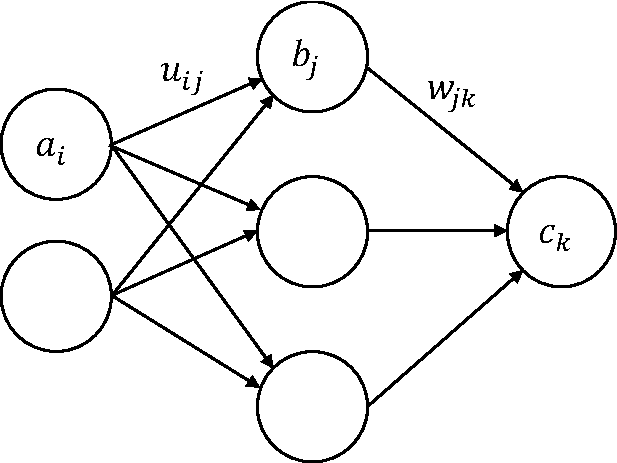
\includegraphics[width=7cm]{fig/DeepNet.pdf}
 \end{center}

%%%%%%%%%%%%%%%%%%%%%%%%%%%%%%%%%%%%%%
%%%%%  BEGINNING OF SUBPROBLEMS LIST
\begin{enumerate}

% Subproblem description
\examproblempart{ For $g(x)=\sigma(x)=\frac{1}{1+e^{-x}}$, compute the derivative $g'(x)$ of $g(x)$ as a function of $\sigma(x)$.}
\bookletskip{0}   %in inches

% Solution box 
 \framebox[14.7cm][l]{
 \begin{minipage}[b]{14.7cm}
\inbooklet{Your answer: \backpropStudSolA}
  
 \solution{\backpropSolA}

 \end{minipage}
 }

% Subproblem description
\examproblempart{ We denote by $\delta_{k}=\frac{\partial E}{\partial h_{k}}$ the error signal of neuron $k$ in the second linear layer of the network. Compute $\delta_{k}$ as a function of $c_k$, $t_k$, $g'$ and $h_k$.\\ }
\bookletskip{0}   %in inches

% Solution box 
 \framebox[14.7cm][l]{
 \begin{minipage}[b]{14.7cm}
\inbooklet{Your answer: \backpropStudSolB}
  
 \solution{\backpropSolB}

 \end{minipage}
 }

% Subproblem description
\examproblempart{ Compute $\frac{\partial E}{\partial w_{jk}}$. Use $\delta_k$ and $b_j$.\\}
\bookletskip{0.0}   %in inches

% Solution box 
 \framebox[14.7cm][l]{
 \begin{minipage}[b]{14.7cm}
 \inbooklet{Your answer: \backpropStudSolC}
  
 \solution{\backpropSolC}
  \end{minipage}
  }

% Subproblem description
\examproblempart{Compute $\frac{\partial E}{\partial f_{k}}$. Use $\delta_{k}$.\\}
\bookletskip{0.0}   %in inches

% Solution box 
 \framebox[14.7cm][l]{
 \begin{minipage}[b]{14.7cm}
 \inbooklet{Your answer: \backpropStudSolD}
  
 \solution{\backpropSolD}
 \end{minipage}
 }

% Subproblem description
\examproblempart{We denote by $\psi_{j}=\frac{\partial E}{\partial z_{j} }$ the error signal of neuron $j$ in the first linear layer of the network. Compute $\psi_{j}$ as a function of $\delta_{k}$, $w_{jk}$, $g'$ and $z_{j}$.\\ }
\bookletskip{0}   %in inches

% Solution box 
 \framebox[14.7cm][l]{
 \begin{minipage}[b]{14.7cm}
 \inbooklet{Your answer: \backpropStudSolE}
  
 \solution{\backpropSolE}
 \end{minipage}
 }
 
 
 % Subproblem description
\examproblempart{Compute $\frac{\partial E}{\partial u_{ij}}$. Use $\psi_{j}$ and $a_i$.\\ }
\bookletskip{0}   %in inches

% Solution box 
 \framebox[14.7cm][l]{
 \begin{minipage}[b]{14.7cm}
 \inbooklet{Your answer: \backpropStudSolF}
  
 \solution{\backpropSolF}
 \end{minipage}
 }
 
 
  % Subproblem description
\examproblempart{Compute $\frac{\partial E}{\partial e_{j}}$. Use $\psi_{j}$.\\ }
\bookletskip{0}   %in inches

% Solution box 
 \framebox[14.7cm][l]{
 \begin{minipage}[b]{14.7cm}
 \inbooklet{Your answer: \backpropStudSolH}
  
 \solution{\backpropSolH}
 \end{minipage}
 }
 
 
 %%%%%%%%%%%% END OF SUBPROBLEMS LIST

\end{enumerate}
%\bookletpage
%\input{MRF}
%\bookletpage
%% !TEX root = exam.tex
\ifthenelse{\equal{\type}{booklet}}{
\newcommand{\GMMkMeansStudSolA}{
%%%%%%%%%%%%%%%%%%%%%%%%%%%%%%%%%%%%
%%
%%.   YOUR SOLUTION FOR PROBLEM A BELOW THIS COMMENT
%%
%%%%%%%%%%%%%%%%%%%%%%%%%%%%%%%%%%%%
Unsupervised. It doesn't use any kind of label.
}

\newcommand{\GMMkMeansStudSolB}{
%%%%%%%%%%%%%%%%%%%%%%%%%%%%%%%%%%%%
%%
%%.   YOUR SOLUTION FOR PROBLEM A BELOW THIS COMMENT
%%
%%%%%%%%%%%%%%%%%%%%%%%%%%%%%%%%%%%%
By adding a constraint on $r_{ik}$. We would want $r_{ik}$ to be 1 for one, and only one, $k$ for each $i$. So, our constraints can be written as:
\[ r_{ik} \in \{0, 1\} \hspace{0.3cm} \forall i \in \{1, 2, \cdots, D \}, \forall r \in \{1, 2, \cdots, K \} \eqno{(1)}\]
\[ \sum_{k=1}^K r_{ik} = 1 \hspace{0.3cm} \forall i \in \{1, 2, \cdots, D \} \eqno{(2)} \]

Additional to those constraints we could also specify a constraint to ensure the active $k$ is the one corresponding to the closest center:
\[ r_{ik} = \delta\left( k = \argmin_j ||x_i - \mu_j ||^2 \right) \]
}

\newcommand{\GMMkMeansStudSolC}{
%%%%%%%%%%%%%%%%%%%%%%%%%%%%%%%%%%%%
%%
%%.   YOUR SOLUTION FOR PROBLEM A BELOW THIS COMMENT
%%
%%%%%%%%%%%%%%%%%%%%%%%%%%%%%%%%%%%%
Replace the integrity constraint $r_{ik} \in \{0, 1\}$ with $r_{ik} \in [0, 1]$ and ignore the $\delta$ function.
}

\newcommand{\GMMkMeansStudSolD}{
%%%%%%%%%%%%%%%%%%%%%%%%%%%%%%%%%%%%
%%
%%.   YOUR SOLUTION FOR PROBLEM A BELOW THIS COMMENT
%%
%%%%%%%%%%%%%%%%%%%%%%%%%%%%%%%%%%%%
Using the Elbow method\footnote{\url{https://en.wikipedia.org/wiki/Elbow_method_(clustering)}} we can say that $k = 5$ is the best choice because after that the cost decrease is too small.
}

\newcommand{\GMMkMeansStudSolE}{
%%%%%%%%%%%%%%%%%%%%%%%%%%%%%%%%%%%%
%%
%%.   YOUR SOLUTION FOR PROBLEM A BELOW THIS COMMENT
%%
%%%%%%%%%%%%%%%%%%%%%%%%%%%%%%%%%%%%
The basic $k$-means, using Euclidean distance, is certainly not enough to cluster the provided data. The reason for this is that $k$-means tries to find non-overlapping spherical clusters. This is a consequence of using Euclidean distance and not of the $k$-means algorithm per se.  But $k$-means can be used with a whole family of distance functions. There are distance functions that are kernel based that can effectively identify clusters in this data. A Gaussian Kernel based distance is one of them \footnote{\url{https://sites.google.com/site/dataclusteringalgorithms/kernel-k-means-clustering-algorithm}}, this is sometimes referred as Spectral clustering.
}

%\newcommand{\GMMkMeansStudSolF}{
%%%%%%%%%%%%%%%%%%%%%%%%%%%%%%%%%%%%%
%%%
%%%.   YOUR SOLUTION FOR PROBLEM A BELOW THIS COMMENT
%%%
%%%%%%%%%%%%%%%%%%%%%%%%%%%%%%%%%%%%%
%}
 %The students have to fill this file to print the solution
}{
\input{GMMkMeans_OurSolution} %This file will not be provided to students since it contains the solution
}

% Problem Explanation:
% - first argument is the number of points
% - second argument is the title and the text
\examproblem{10}{K-Means\\}


%%%%%%%%%%%%%%%%%%%%%%%%%%%%%%%%%%%%%%
%%%%%  BEGINNING OF SUBPROBLEMS LIST

\begin{enumerate}

 % Subproblem description
\examproblempart{Mention if K-Means is a supervised or an un-supervised method.
 \\}

\bookletskip{0.0}   %in inches

% Solution box
 \framebox[14.7cm][l]{
 \begin{minipage}[b]{14.7cm}
 \inbooklet{Your answer: \GMMkMeansStudSolA}
  
 \solution{\GMMkMeansSolA}
 \end{minipage}
 }
 
  % Subproblem description
\examproblempart{Assume that you are trying to cluster data points $x_{i}$  for $ i \in \{1,2 \dots D\}$ into K clusters each with center $\mu_{k}$  where $ k \in \{1,2, \dots K \}$. The objective function for doing this clustering involves minimizig the euclidean distance between the points and the cluster centers. It is given by  \begin{equation*}
\min\limits_{\mu} \min\limits_{r}\sum\limits_{i \in D} \sum\limits_{k =1}^{K} \frac{1}{2} r_{ik} ||x_{i} -\mu_{k}||_{2}^{2} \\
 \end{equation*} \\ How do you ensure hard assignemnt of one data point to one and only one cluster at a given time? Note: By hard assignment we mean that your are 100 \% sure that a point either belongs or not belongs to a cluster.\\}

\bookletskip{0.0}   %in inches

% Solution box
 \framebox[14.7cm][l]{
 \begin{minipage}[b]{14.7cm}
 \inbooklet{Your answer: \GMMkMeansStudSolB}
  
 \solution{\GMMkMeansSolB }
 \end{minipage}
 }
 
% Subproblem description
\examproblempart{What changes must you do in your answer of part b, to make the hard assingment into a soft assignment? Note: By soft assignment we mean that your are  sure that a point either belongs or not belongs to a cluster with some probability.\\}

\bookletskip{0.0}   %in inches

% Solution box
 \framebox[14.7cm][l]{
 \begin{minipage}[b]{14.7cm}
 \inbooklet{Your answer: \GMMkMeansStudSolC}
  
 \solution{\GMMkMeansSolC}
 \end{minipage}
 }
 
 % Subproblem description
 \examproblempart{Looking at the following plot, what is the best choice for number of clusters?}
  \begin{center}
 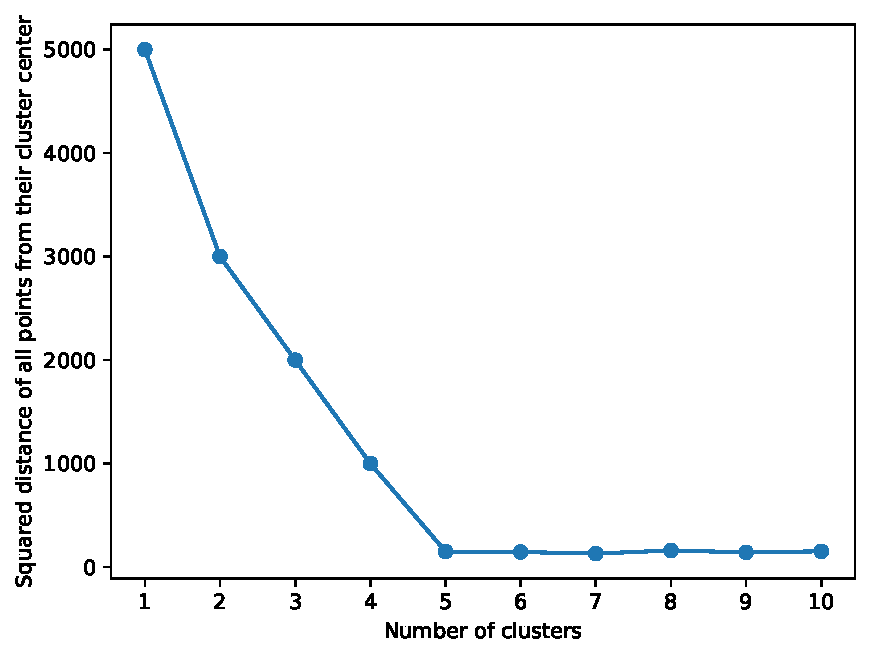
\includegraphics[width=8cm]{fig/cluster.pdf}
 \end{center}
\bookletskip{0.0}   %in inches

% Solution box
 \framebox[14.7cm][l]{
 \begin{minipage}[b]{14.7cm}
 \inbooklet{Your answer: \GMMkMeansStudSolD}
  
 \solution{\GMMkMeansSolD}
 \end{minipage}
 }

% Subproblem description
 \examproblempart{Would K-Means be an effecient algorithm to cluster the following data? Explain your answer in a couple of lines.}
  \begin{center}
 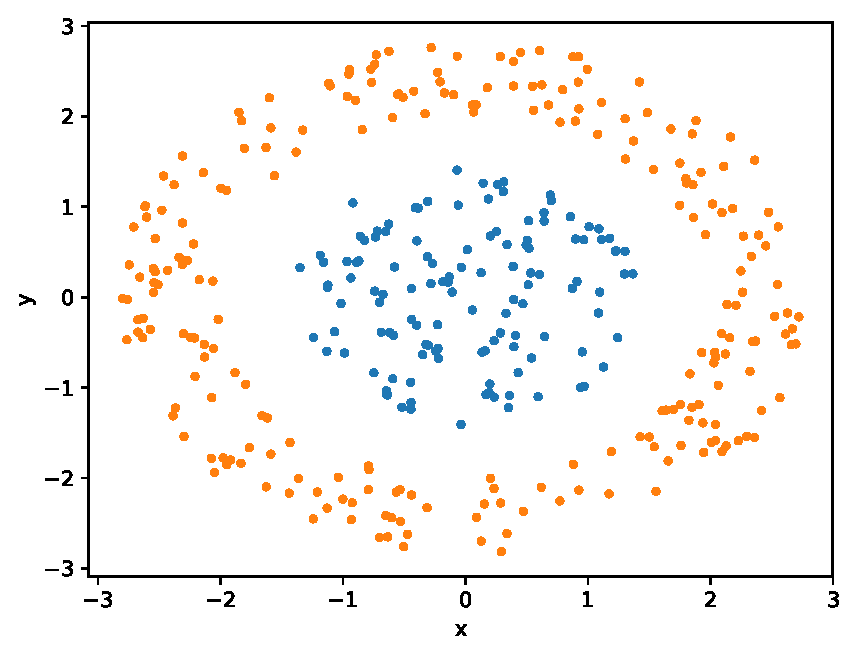
\includegraphics[width=8cm]{fig/concentric.pdf}
 \end{center}
\bookletskip{0.0}   %in inches

% Solution box
 \framebox[14.7cm][l]{
 \begin{minipage}[b]{14.7cm}
 \inbooklet{Your answer: \GMMkMeansStudSolE}
  
 \solution{\GMMkMeansSolE}
 \end{minipage}
 }
 
 %}
 
  %%%%%%%%%%%% END OF SUBPROBLEMS LIST
  
 \end{enumerate}
%\bookletpage
%\input{VAE}
%\bookletpage
%\input{VAE2}
%\bookletpage
%\input{GAN}
%\bookletpage
%\input{GAN2}
%\bookletpage
%\input{MDP}
%\bookletpage
% !TEX root = exam.tex
\newcommand{\QLearnStudSolA}{
%%%%%%%%%%%%%%%%%%%%%%%%%%%%%%%%%%%%
%%
%%.   YOUR SOLUTION FOR PROBLEM A BELOW THIS COMMENT
%%
%%%%%%%%%%%%%%%%%%%%%%%%%%%%%%%%%%%%
\[
	Q^*(s, a) = \sum_{s\prime \in S} P(s\prime | s, a) \left[
		R(s, a, s\prime) + \max_{a\prime \in \mathcal{A}_{s\prime}} Q^*(s\prime, a\prime)	
	\right]
\]
}

\newcommand{\QLearnStudSolB}{
%%%%%%%%%%%%%%%%%%%%%%%%%%%%%%%%%%%%
%%
%%.   YOUR SOLUTION FOR PROBLEM A BELOW THIS COMMENT
%%
%%%%%%%%%%%%%%%%%%%%%%%%%%%%%%%%%%%%
\[
	Q(s, a) \leftarrow (1 - \alpha) \cdot Q(s, a) + \alpha \cdot \left(
		R(s, a, s\prime) + \gamma \cdot \max_{a\prime \in \mathcal{A}_{s\prime}} Q(s\prime, a\prime)	
	\right)
\]
}

\newcommand{\QLearnStudSolC}{
%%%%%%%%%%%%%%%%%%%%%%%%%%%%%%%%%%%%
%%
%%.   YOUR SOLUTION FOR PROBLEM A BELOW THIS COMMENT
%%
%%%%%%%%%%%%%%%%%%%%%%%%%%%%%%%%%%%%
Since we are assuming the environment is stochastic given a \textbf{known} state and action pair, it may be the case that there is another action that yields a better reward from the same state. $\epsilon$-greedy allows the agent to \textit{explore} the environment in hope of finding better actions that the ones currently seen. 

You could see $\epsilon$ as a control of the tradeoff between exploitation (always performing the best action) and exploration (potentially resulting in trying new actions).
}

\newcommand{\QLearnStudSolD}{
%%%%%%%%%%%%%%%%%%%%%%%%%%%%%%%%%%%%
%%
%%.   YOUR SOLUTION FOR PROBLEM A BELOW THIS COMMENT
%%
%%%%%%%%%%%%%%%%%%%%%%%%%%%%%%%%%%%%
The main advantage is that it allows us to approximate the probability $P(s\prime | s, a)$ which is, more often than not, unknown. Another reason is that by keeping track of the past experiences ($(s, a, s\prime, r)$ tuples) and sampling randomly it removes the correlation in the observed sequence of states, as explained in \url{https://datascience.stackexchange.com/questions/20535/understanding-experience-replay-in-reinforcement-learning}
}

\newcommand{\QLearnStudSolE}{
%%%%%%%%%%%%%%%%%%%%%%%%%%%%%%%%%%%%
%%
%%.   YOUR SOLUTION FOR PROBLEM A BELOW THIS COMMENT
%%
%%%%%%%%%%%%%%%%%%%%%%%%%%%%%%%%%%%%
Given the updates performed, and shown in the tables above, we can use 
\begin{displaymath}
\pi (s) = \text{arg}\max_{a \in \mathcal{A}_s} Q^*(s, a)
\end{displaymath}

where $A_s = \{a_1, a_2\}$ for $s \in \{ S_1, S_2 \}$. So

\begin{displaymath}
	\pi(S_1) = \text{arg}\max_{a \in \mathcal{A}_{S_1}} Q^*(S_1, a) = a_1
\end{displaymath}

\begin{displaymath}
	\pi(S_2) = \text{arg} \max_{a \in \mathcal{A}_{S_2}} Q^*(S_2, a) = a_1
\end{displaymath}
}
 %The students have to fill this file to print the solution


% Problem Explanation:
% - first argument is the number of points
% - second argument is the title and the text
\examproblem{13}{Q-Learning
}

%%%%%%%%%%%%%%%%%%%%%%%%%%%%%%%%%%%%%%
%%%%%  BEGINNING OF SUBPROBLEMS LIST
\begin{enumerate}

% Subproblem description
\examproblempart{State the Bellman optimality principle as a function of the optimal Q-function $Q^{*}(s,a)$, the expected reward function $R(s,a,s')$ and the transition probability $P(s'|s,a)$, where $s$ is the current state, $s'$ is the next state and $a$ is the action taken in state $s$.\\
}
\bookletskip{0}   %in inches

% Solution box 
  \framebox[14.7cm][l]{
 \begin{minipage}[b]{14.7cm}
 \inbooklet{Your answer: \QLearnStudSolA}
  
 \solution{\QLearnSolA}
 \end{minipage}
 }
 
% Subproblem description 
 \examproblempart{In case the transition probability $P(s'|s,a)$ and the expected reward $R(s,a,s')$  are unknown, a stochastic  approach is used to approximate the optimal Q-function. After observing a transition of the form $(s,a,r,s')$, write down the update of the Q-function at the observed state-action pair $(s,a)$ as a function of the learning rate $\alpha$, the discount factor $\gamma$, $Q(s,a)$ and $Q(s',a')$.\\

}
\bookletskip{0}   %in inches

% Solution box 
  \framebox[14.7cm][l]{
 \begin{minipage}[b]{14.7cm}
 \inbooklet{Your answer: \QLearnStudSolB}
  
 \solution{\QLearnSolB}
 \end{minipage}
 }

% Subproblem description
\examproblempart{What is the advantage of an epsilon-greedy strategy? \\}
\bookletskip{0.0}   %in inches
 
% Solution box  
   \framebox[14.7cm][l]{
 \begin{minipage}[b]{14.7cm}
 \inbooklet{Your answer: \QLearnStudSolC}
  
 \solution{\QLearnSolC}
 \end{minipage}
 }
 
% Subproblem description 
 \examproblempart{What is the advantage of using a replay-memory?  \\}
\bookletskip{0.0}   %in inches
 
% Solution box  
   \framebox[14.7cm][l]{
 \begin{minipage}[b]{14.7cm}
 \inbooklet{Your answer: \QLearnStudSolD}
  
 \solution{\QLearnSolD}
 \end{minipage}
 }
 

 
\bookletpage
% Subproblem description
 \examproblempart{Consider a system with two states $S_{1}$ and $S_{2}$ and two actions $a_{1}$ and $a_{2}$. You perform actions and observe the rewards and transitions listed below. Each step lists the current state, reward, action and resulting transition as: $S_{i};  R=r; a_{k}: S_{i} \rightarrow S_{j}  $. Perform Q-learning using a learning rate of $\alpha=0.5$ and a discount factor of $\gamma=0.5$ for each step by applying the formula from part (b). The Q-table entries are initialized to zero.  Fill in the tables below corresponding to the following four transitions. What is the optimal policy after having observed the four transitions?}
 
 \begin{enumerate}
\item $S_{1}$; $R=-10$; $a_{1}:S_{1}\rightarrow S_{1}$
\item  $S_{1}$; $R=-10$; $a_{2}:S_{1}\rightarrow S_{2}$
\item $S_{2}$; $R=18.5$; $a_{1}:S_{2}\rightarrow S_{1}$
\item $S_{1}$; $R=-10$; $a_{2}:S_{1}\rightarrow S_{2}$

\end{enumerate}

 

\bookletskip{0}   %in inches


\begin{table}[h]
\small       
\begin{tabular}[t]{|c c c|}
\hline
$Q$ & $S_{1}$ & $S_{2}$  \\ \hline
$a_{1}$&-5&0\\ \hline
$a_{2}$& 0 & 0\\ \hline
\end{tabular}
\hfill
\begin{tabular}[t]{|c c c|}
\hline
$Q$ & $S_{1}$ & $S_{2}$  \\ \hline
$a_{1}$&-5&0\\ \hline
$a_{2}$&-5&0\\ \hline
\end{tabular}
\hfill
\begin{tabular}[t]{|c c c|}
 \hline
 $Q$ & $S_{1}$ & $S_{2}$  \\ \hline
 $a_{1}$&-5&8\\ \hline
 $a_{2}$&-5&0 \\ \hline
 \end{tabular}
 \hfill
 \begin{tabular}[t]{|c c c|}
 \hline
 $Q$ & $S_{1}$ & $S_{2}$  \\ \hline
 $a_{1}$&-5&8\\ \hline
 $a_{2}$&-5.5&0 \\ \hline
\end{tabular}
\end{table}

% Solution box 
  \framebox[14.7cm][l]{
 \begin{minipage}[b]{14.7cm}
 \inbooklet{Your answer: \QLearnStudSolE}
  
 \solution{\QLearnSolE}
 \end{minipage}
 }
 
%%%%%%%%%%%% END OF SUBPROBLEMS LIST

\end{enumerate}

%%%%%%%%%%%% END OF PROBLEMS LIST

\end{enumerate}
\end{document}

